\documentclass[class=report, crop=false, 12pt,a4paper]{standalone}
\usepackage{enumitem}
\usepackage{multicol}
\usepackage{graphicx}
\usepackage{float}
\usepackage{amsmath}
\usepackage{amssymb}
\usepackage{mathtools}
\usepackage{siunitx}
\usepackage{commath}
\usepackage{array}
\usepackage{natbib}
\usepackage[a4paper,width=150mm,top=25mm,bottom=25mm]{geometry}
\setlength{\parindent}{0pt}
\setlength{\parskip}{1em}
\raggedbottom
\begin{document}
\chapter{Faulted Networks}
\begin{itemize}
	\item Introducing the concept of unbalanced networks
	\item Using impedance diagrams for fault calculations
\end{itemize}
\subsection{Symmetrical faults recap}
In a power system the most significant fault that can occur is when all three-phases short together. This is a symmetrical or balanced fault. The MVA Fault Level defines the maximum MVA that the system is subjected to when a symmetrical fault event occurs. The fault level is usually expressed in MVA (or a corresponding per-unit value). The maximum fault current can be calculated using the MVA Fault Level and the nominal Voltage Rating at the fault location.
\section{Unbalanced faults}
\subsection{Types of `unbalanced faults'}
Unsymmetrical faults - currents and voltages are not balanced in each phase:
\begin{itemize}
	\item Single line to ground
	\item Line to line
	\item Double line to ground
	\item Single phase open circuit
	\item Dounle phase open circuit
\end{itemize}
For each short-circuit, the fault can be bolted (a zero impedance fault) or have a fault impedance known as Zf.
\begin{figure}[H]
	\centering
	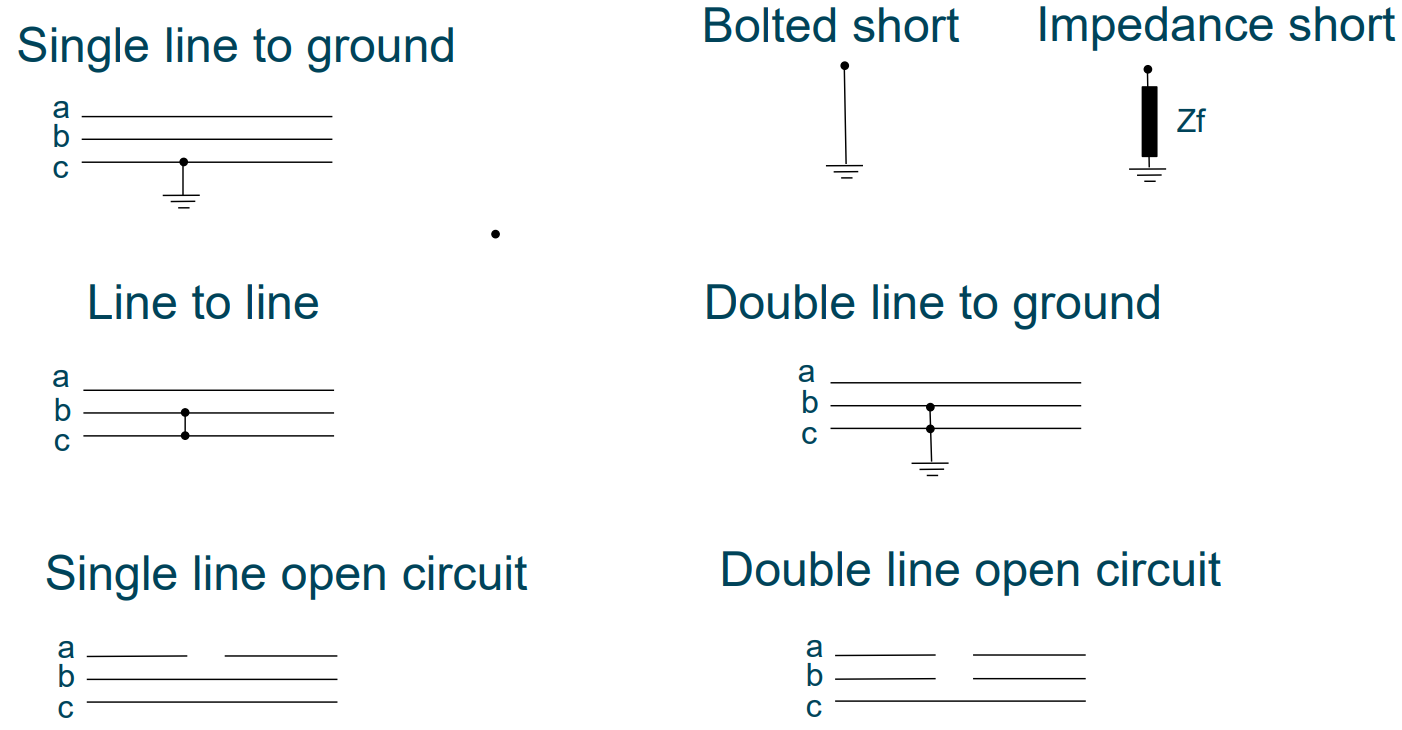
\includegraphics[width = \textwidth]{../img/figure20.png}
	\caption{Unsymmetrical/unbalanced faults.}
\end{figure}
\subsection{List of possible faults}
\begin{itemize}
	\item Three phase symmetrical fault L-L-L
	\item Three phase symmetrical fault L-L-L-G
	\item Line to line fault
	\item Double line to ground fault
	\item Single line to ground fault
	\item Single line open circuit
	\item Double line open circuit
\end{itemize}
The most common fault is the single line to ground fault. The worst fault is a three-phase to ground fault (L-L-L-G or L-L-L).
\begin{figure}[H]
	\centering
	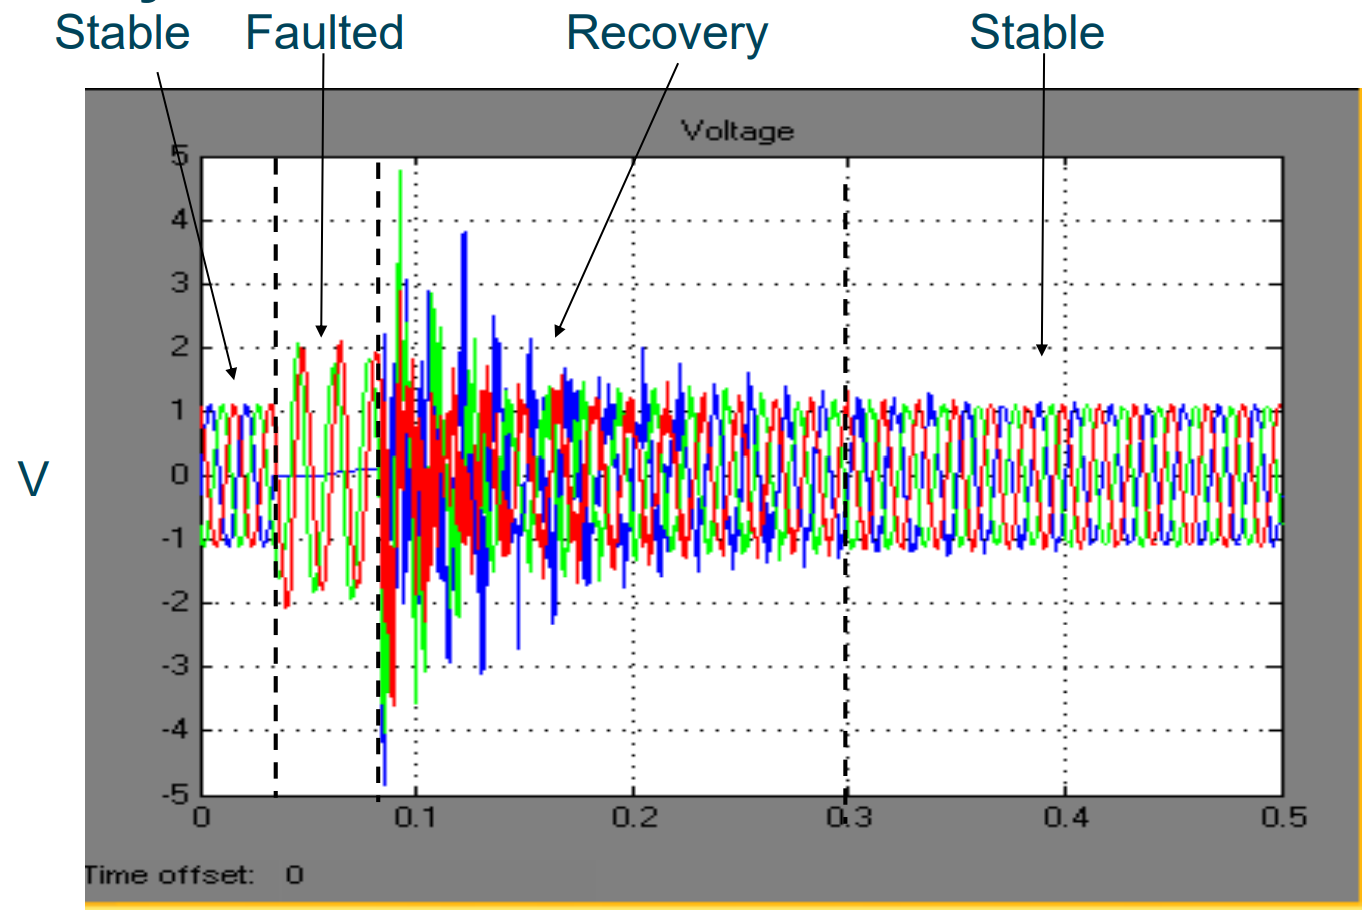
\includegraphics[width = \textwidth]{../img/figure21.png}
	\caption{Unsymmetrical/unbalanced fault graph.}
\end{figure}
We see the blue phase go to ground (0V) and the other two phases increase in voltage and are no longer \SI{120}{\degree} out of phase with each other. 
\subsection{Method of analysis}
Each phase is experiencing something different i.e. what is happening on one phase is not what is happening on the other. RMS voltages and currents are unbalanced.
\begin{gather}
	V_a \neq V_b \neq V_c \textrm{ nor } I_a \neq I_b \neq I_c
\end{gather}
The presumption that we used for symmetrical faults (the same equivalent circuit for each phase) is not valid in the unsymmetrical/unbalanced case. For the unbalanced case it is necessary to use a different method. We use `Fortescues's Theorem'.
\subsection{Fortescue's Theorem}
Fortescue's Theorem says:
\begin{quote}
	Three unbalanced phasors in a multi-phase electrical system can be resolved into a set of balanced phasors consisting of:
\end{quote}
\begin{itemize}
	\item Positive-sequence components
	\item Negative-sequence components
	\item Zero sequence components
\end{itemize}
\begin{align}
	V_{line} &= V_{positive} + V_{negative} + V_{zero}\\
	I_{line} &= I_{positive} + I_{negative} + I_{zero}
\end{align}
\subsection{Positive sequence components}
For a three-phase system there are three balanced phasors:
\begin{itemize}
	\item Equal in magnitude
	\item Displaced from each other by \SI{120}{\degree}
	\item Have phase sequence a-b-c
	\item Usually referred to as $V_{a1}$, $V_{b1}$, $V_{c1}$
\end{itemize}
\subsection{Negative sequence components}
For a three-phase system there are three balanced phasors:
\begin{itemize}
	\item Equal in magnitude
	\item Displaced from each other by \SI{120}{\degree}
	\item Have phase sequence a-c-b
	\item Usually referred to as $V_{a2}$, $V_{b2}$, $V_{c2}$
\end{itemize}
\subsection{Zero sequence components}
For a three-phase system there are three balanced phasors:
\begin{itemize}
	\item Equal in magnitude
	\item Zero phase displacement
	\item No phase sequence
	\item Usually referred to as $V_{a0}$, $V_{b0}$, $V_{c0}$
\end{itemize}
\begin{figure}[H]
	\centering
	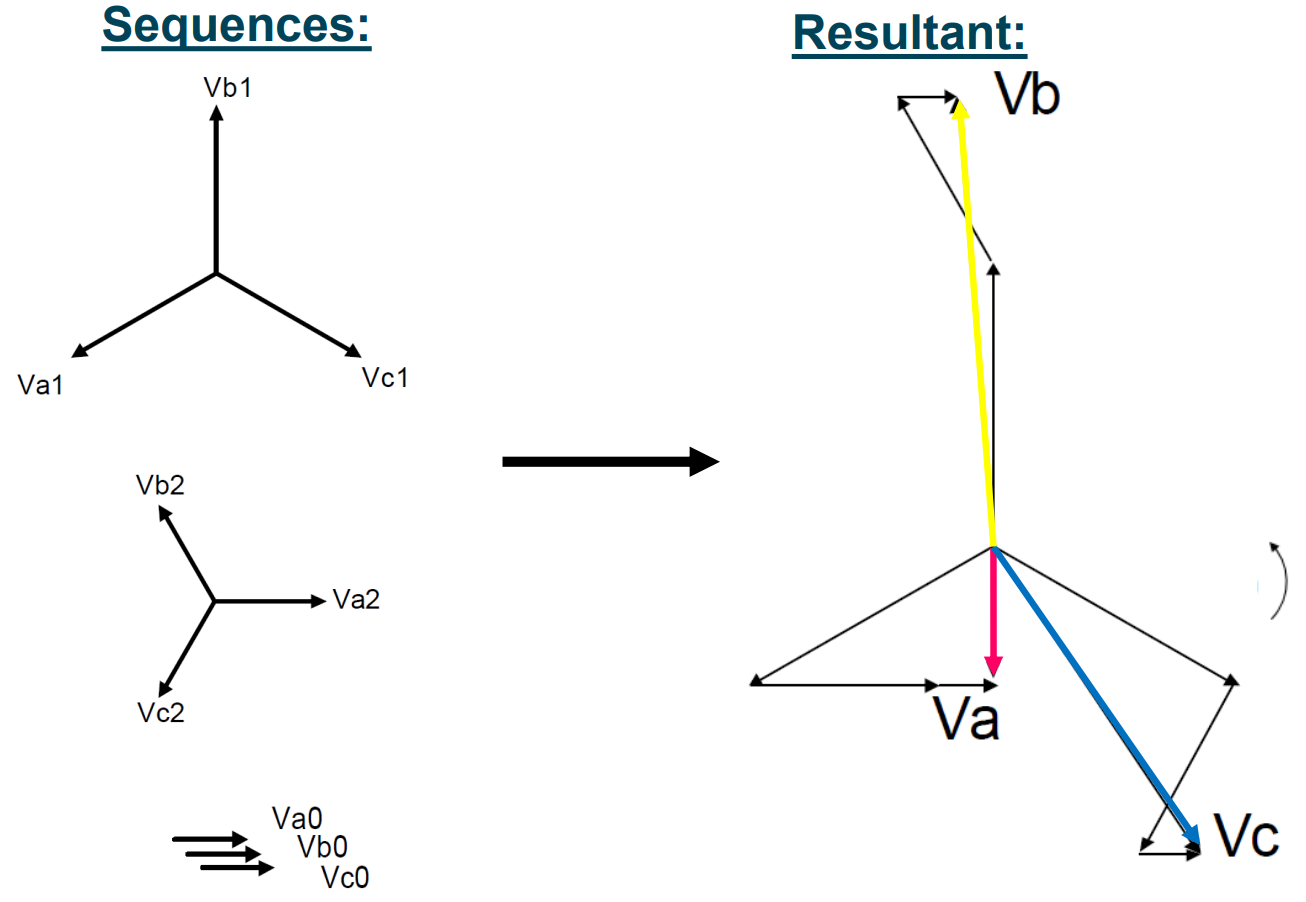
\includegraphics[width = \textwidth]{../img/figure22.png}
	\caption{Sequence components and phase relationship.}
\end{figure}
\begin{figure}[H]
	\centering
	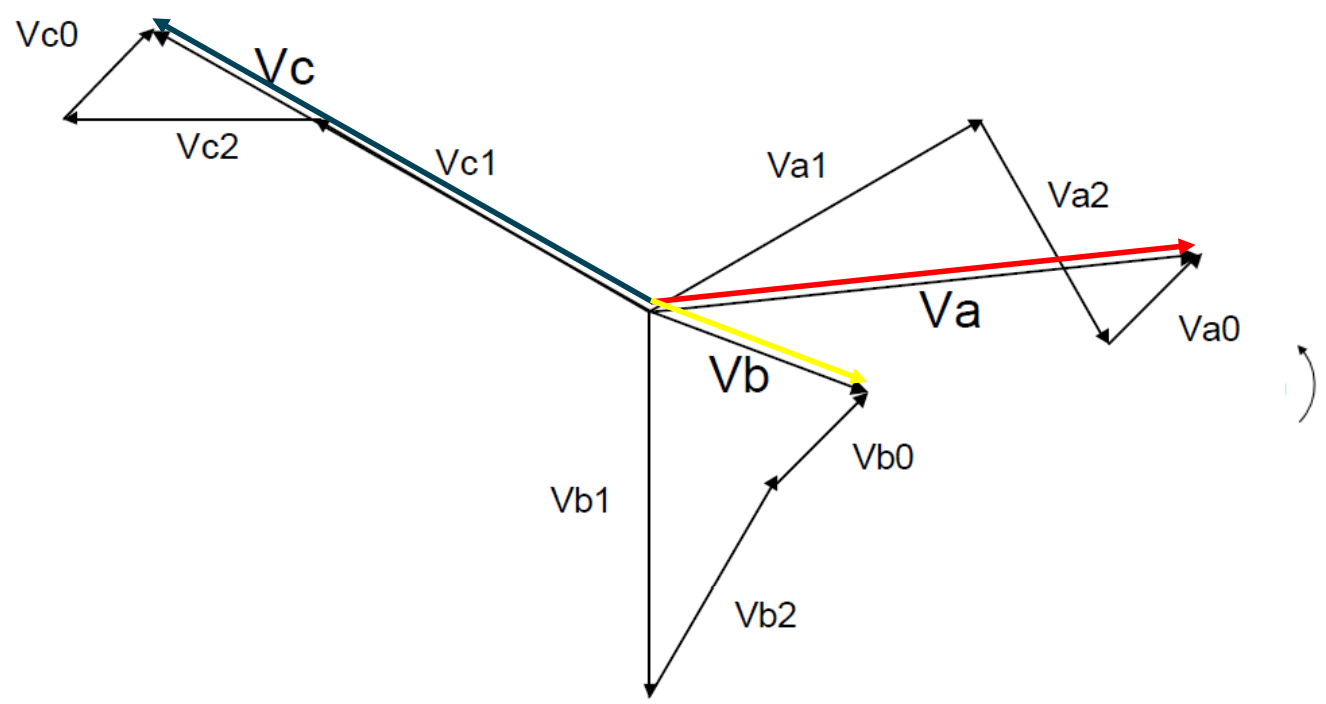
\includegraphics[width = \textwidth]{../img/figure23.png}
	\caption{Sequence components 2.}
\end{figure}
\subsection{Summing sequence components}
Original phasors are the sum of their components
\begin{align}
	V_a &= V_{a0} + V_{a1} + V_{a2}\\
	V_b &= V_{b0} + V_{b1} + V_{b2}\\
	V_c &= V_{c0} + V_{c1} + V_{c2}
\end{align}
Hence:
\begin{gather}
	\textrm{Line} = \sum \textrm{sequence components}
\end{gather}
In balanced/symmetrical networks in multi-phase systems then only positive sequence components are present.
\subsection{Note about grounding/earthing}
How a system is grounded has a major impact on fault current. Zero sequence current can only flow when the start point of the source is tied to ground / earth directly or via an impedance Ze. 
\begin{figure}[H]
	\centering
	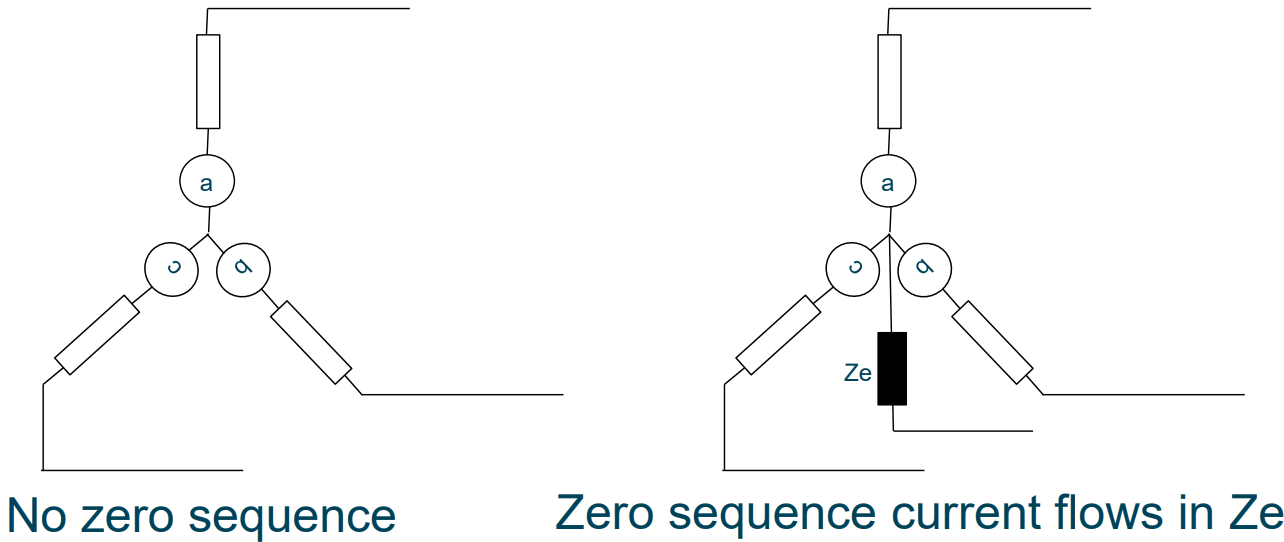
\includegraphics[width = \textwidth]{../img/figure24.png}
	\caption{Grounding/earthing.}
\end{figure}
We can see the virtual/floating star point on the sequence on the left. Normally, this is left floating on ship systems for example. The star point can be connected to ground (unusual for generators) or we can add an impedance to the star point connection. This is because the star point is not always 0V under a fault condition. Hence, by including an earth impedance, we can limit current flow.

Zero sequence current flows can only happen if we have a connection to ground. In floating star point connections, we cannot have zero sequence current flows.
\begin{figure}[H]
	\centering
	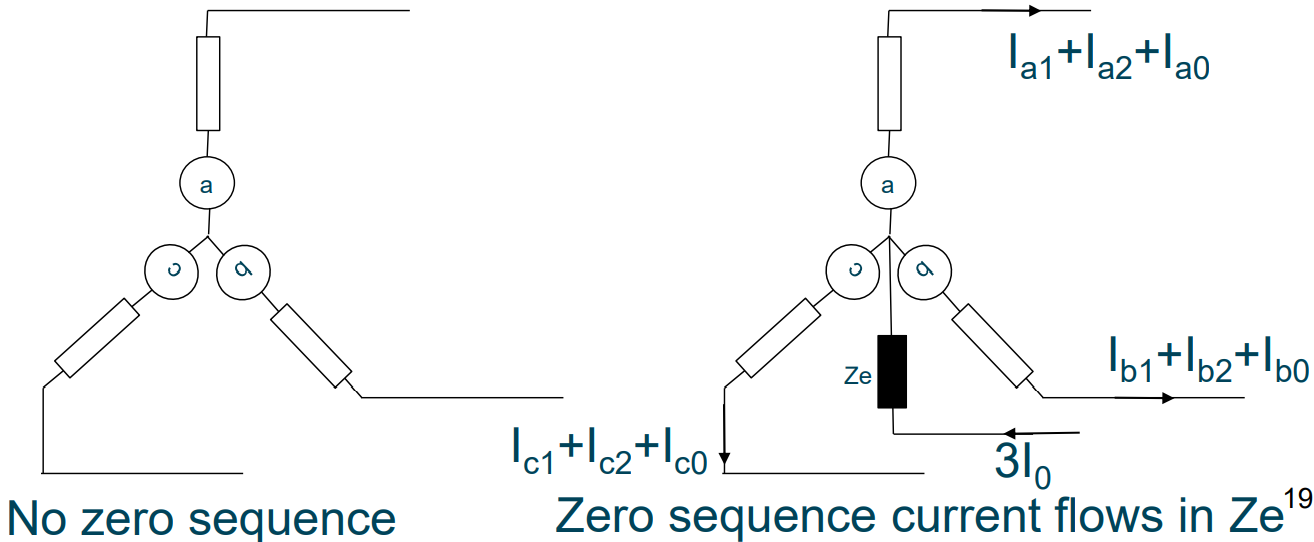
\includegraphics[width = \textwidth]{../img/figure25.png}
	\caption{Currents during grounded star point.}
\end{figure}
\begin{figure}[H]
	\centering
	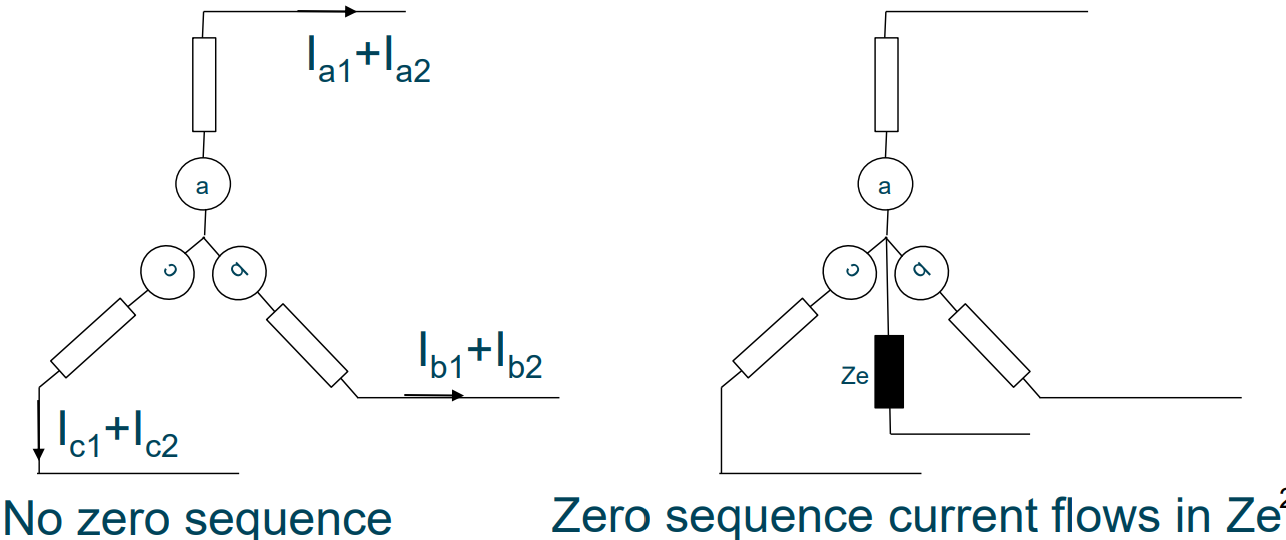
\includegraphics[width = \textwidth]{../img/figure26.png}
	\caption{Currents during floating star point.}
\end{figure}
\subsection{The operator `a'}
Let us define an operator that rotates a phasor by \SI{120}{\degree}:
\begin{gather}
	a = 1\angle \SI{120}{\degree} = (-0.5 + j 0.8666)
\end{gather}
\begin{figure}[H]
	\centering
	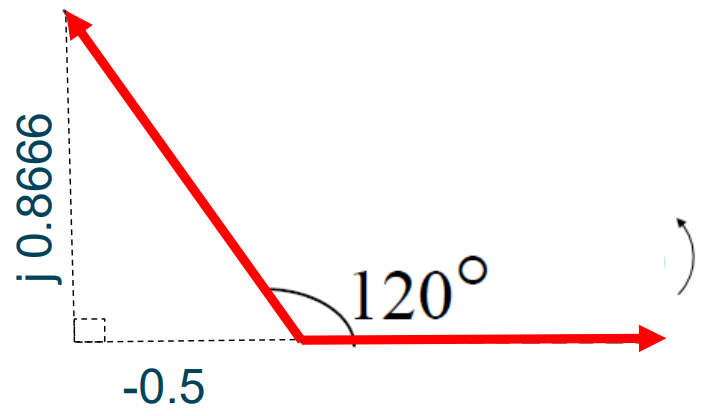
\includegraphics[width = 0.4\textwidth]{../img/figure27.png}
	\caption{`a' operator.}
\end{figure}
\subsection{Expressing phasors $a^2$ and $a^3$}
\begin{gather}
	a^2 = a \times a = \left(1 \angle \SI{240}{\degree}\right) = 1 \angle \SI{-120}{\degree}
\end{gather}
Similarly:
\begin{gather}
	a^3 = \left( 1 \angle \SI{360}{\degree}\right) = 1 \angle \SI{0}{\degree}
\end{gather}
Therefore:
\begin{align}
	a + a^2 + a^3 &= 0\\
	1 + a + a^2 &= 0
\end{align}
\begin{figure}[H]
	\centering
	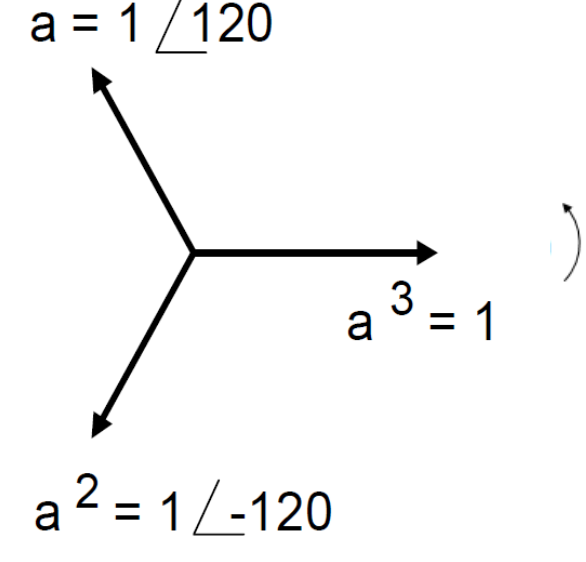
\includegraphics[width = 0.4\textwidth]{../img/figure28.png}
	\caption{`a' phasors.}
\end{figure}
The value of the star point changes with fault conditions.
\subsection{Representation using `a'}
Using the `a' operator then the positive sequence components can be written:
\begin{align}
	V_{a1} &= 1\\
	V_{b1} &= \left(1 \angle -\SI{120}{\degree}\right) = a^2 V_{a1}\\
	V_{c1} &= \left(1 \angle \SI{120}{\degree}\right) = a V_{a1}
\end{align}
In other words we have used the `a' operator to express $V_{b1}$ and $V_{c1}$ in terms of $V_{a1}$. Similarly for the negative sequence, we have:
\begin{align}
	V_{a2} &= 1\\
	V_{b2} &= \left(1 \angle \SI{120}{\degree}\right)V_{a2} = aV_{a2}\\
	V_{b2} &= \left(1 \angle \SI{-120}{\degree}\right)V_{a2} = a^2V_{a2}
\end{align}
In other words we have used the `a' operator to express $V_{b2}$ and $V_{c2}$ in terms of $V_{a2}$. For the zero sequence:
\begin{gather}
	V_{a0} = V_{b0} = V_{c0}
\end{gather}
No need for the operator `a' here as all zero sequence components are in phase!
\begin{figure}[H]
	\centering
	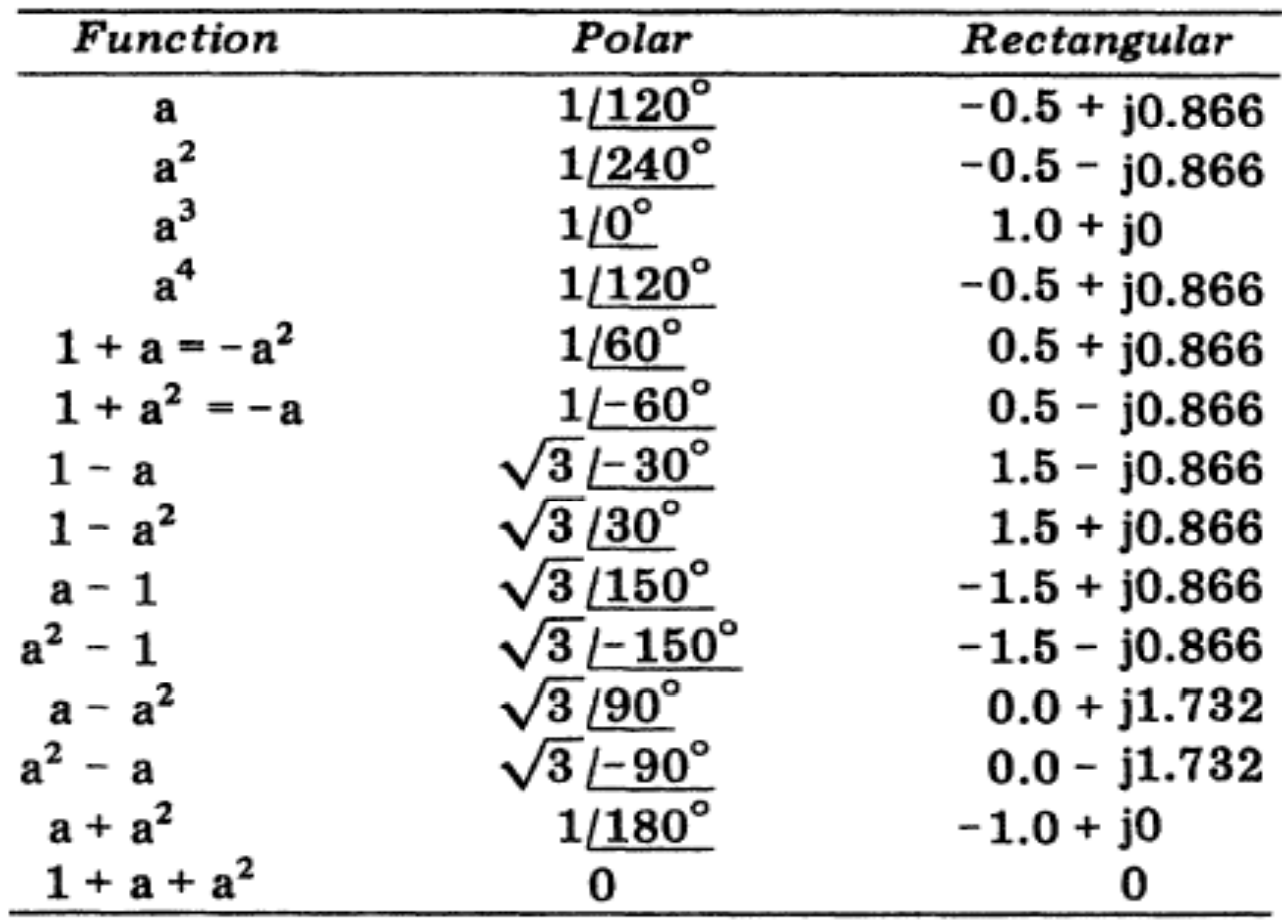
\includegraphics[width = \textwidth]{../img/figure29.png}
	\caption{List of `a' phasors.}
\end{figure}
\subsection{Representing all sequence components in terms of $V_{a}$ sequence components}
\begin{gather}
	\textrm{Line} = \sum \textrm{sequence components}\\
	V_a = V_{a0} + V_{a1} + V_{a2} = V_{a0} + V_{a1} + V_{a2}\\
	V_b = V_{b0} + V_{b1} + V_{b2} = V_{a0} + a^2 V_{a1} + aV_{a2}\\
	V_c = V_{c0} + V_{c1} + V_{c2} = V_{a0} + aV_{a1} + a^2V_{a2}
\end{gather}
\begin{figure}[H]
	\centering
	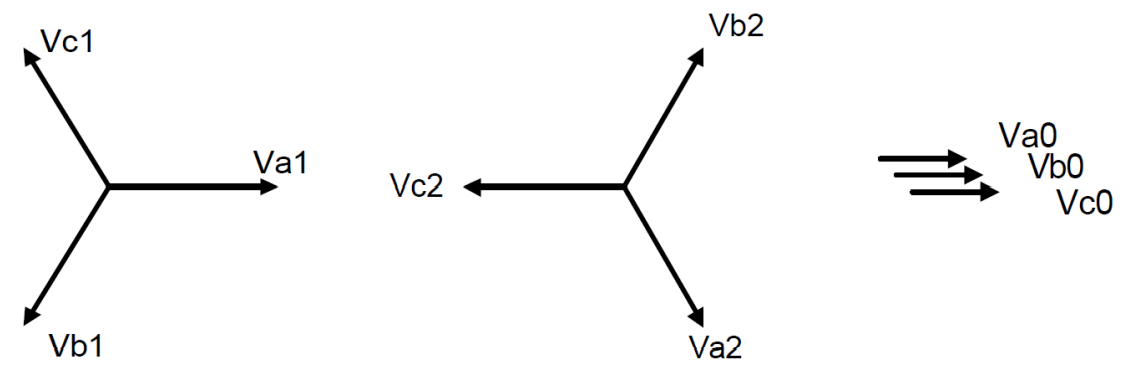
\includegraphics[width = \textwidth]{../img/figure30.png}
	\caption{Phase voltages expressed in terms of $V_{a}$.}
\end{figure}
\subsection{`a' matrix}
\begin{gather}
	\textrm{Line} = \sum \textrm{sequence components}\\
	\begin{bmatrix}
		V_a\\
		V_b\\
		V_c
	\end{bmatrix} = \begin{bmatrix}
		1 & 1 & 1\\
		1 & a^2 & a\\
		1 & a & a^2
	\end{bmatrix}\begin{bmatrix}
		V_{a0}\\
		V_{a1}\\
		V_{a2}
	\end{bmatrix}
\end{gather}
\subsection{Inverse `a' matrix}
The sequences may be described by the `inverse a matrix' and phasors:
\begin{gather}
	\begin{bmatrix}
		V_{a0}\\
		V_{a1}\\
		b_{a2}
	\end{bmatrix} = \frac{1}{3}\begin{bmatrix}
		1 & 1 & 1\\
		1 & a & a^2\\
		1 & a^2 & a
	\end{bmatrix}\begin{bmatrix}
		V_a\\
		V_b\\
		V_c
	\end{bmatrix}
\end{gather}
Where:
\begin{gather}
	A^{-1} = \frac{1}{3}\begin{bmatrix}
		1 & 1 & 1\\
		1 & a & a^2\\
		1 & a^2 & a
	\end{bmatrix}
\end{gather}
\subsection{Example}
A three-phase star connected load is connected across a three-phase balanced supply system. Obtain a set of equations relating the symmetrical components of a line and its phase voltages. Assuming:
\begin{gather}
	V_{ab} = V_a - V_b
\end{gather}
We will do this for one line voltage\dots

Zero sequence. Since:
\begin{gather}
	V_{ab} + V_{bc} + V_{ca} = 0
\end{gather}
then
\begin{gather}
	V_{ab0} + V_{bc0} + V_{ca0} = 0
\end{gather}
In other words there is no change in the zero sequence relationships. Assume balance

Positive sequence:
Choosing $V_{ab}$ then:
\begin{align}
	V_{ab1} &= \frac{1}{3}\left(V_{ab} + aV_{bc} + a^2 V_{ca}\right) \textrm{ from inverse `a' matrix}\\
	&= \frac{1}{3}\left[\left(V_a - V_b\right) + a\left(V_b- V_c\right)+a^2 \left(V_c - V_a\right)\right]\\
	\dots\\
	&= \frac{1}{3}\left[\left(1-a^2\right)\left(V_a + aV_b + a^2 V_c\right)\right]\\
	&= \left(1-a^2\right)V_{a1} \textrm{ from table}\\
	&= \sqrt{3} V_{a1} e^{j30} \textrm{ using exp form}
\end{align}
Negative sequence:
\begin{align}
	V_{ab2} &= \frac{1}{3}\left(V_{ab} + a^2V_{bc} + a V_{ca}\right) \textrm{ from inverse `a' matrix}\\
	&= \frac{1}{3}\left[\left(V_a - V_b\right) + a^2\left(V_b- V_c\right)+a \left(V_c - V_a\right)\right]\\
	\dots\\
	&= \frac{1}{3}\left[\left(1-a\right)\left(V_a + a^2V_b + a V_c\right)\right]\\
	&= \left(1-a\right)V_{a2} \textrm{ from table}\\
	&= \sqrt{3} V_{a2} e^{-j30} \textrm{ using exp form}
\end{align}
\subsection{Sequence components and faults}
\begin{itemize}
	\item This lecture started by considering unsymmetrical faults
	\item The lecture has introduced the method of sequence components and has provided a method analysis of unsymmetrical faults based on Fortescue's theorem
	\item Manipulation of the voltages and currents using the `a' matrix is an important step since this provides the analytical means to analyse unsymmetrical faults from sequence, phase and line perspectives
	\item In the next lecture we will look at unsymmetrical faults by applying this methodology
\end{itemize}
\subsection{Conclusions}
\begin{itemize}
	\item The analysis shown in this session has explained the system analysis methods for `unbalanced faults'
	\item The introuction to the `a' matrix which will be used for relationships between phase and line values and also introuced sequence components
	\item Appreciate the need for positive, negative and zero sequence impedances of different components that make up a power system
\end{itemize}
\end{document}













